\documentclass[11pt]{article}
\usepackage{amsmath}
\usepackage{amssymb}
\usepackage{algpseudocode,algorithm}
\usepackage{graphicx}
\usepackage{psfrag,color}
\usepackage{fullpage}
\usepackage{epsfig}
\usepackage{graphicx}
\usepackage{verbatim}
\usepackage{listings}
\usepackage{subcaption}
\usepackage{float}


\setlength{\topmargin}{-0.7in}
\setlength{\textwidth}{6.5in}
\setlength{\oddsidemargin}{0.0in}
\setlength{\textheight}{10.0in}
\setlength{\parindent}{0in}

\renewcommand{\baselinestretch}{1.2}
\renewcommand\arraystretch{1.5}
\newcommand{\problem}[1]{ \medskip \pp $\underline{\rm Problem\ #1}$\\ }


\pagestyle{empty}

\def\pp{\par\noindent}


\begin{document}

\begin{flushright}
{\bf STAT GR5703---Spring 2020}
\end{flushright}
\begin{flushleft}
Group: Zining Fan, Mutian Wang, Siyuan Wang\\
UNI: zf2234, mw3386, sw3418\\
\end{flushleft}

\bigskip
\centerline{\bf Graded Homework 1 - Exercise 4}

\bigskip
\begin{enumerate}
%4.1
\item 
Fitting a straight line to the data seems reasonable, since there seems to be a positive linear relationship between cirrhosis mortality rate (``cirrhosis'') and liquor consumption per capita (``liquor''). Yet the data points look somewhat dispersed, so we guess $R^2$ might not be very good.

\begin{center}
  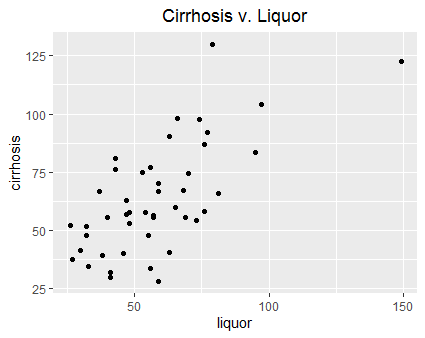
\includegraphics[width=0.7\linewidth]{Q4_1.png}
\end{center}

%4.2
\item 
Cirrhosis mortality rate is the response variable.

%4.3
\item
We expect the two parameters to have the same sign, because from the scatter plot we can clearly see a positive correlation between cirrhosis and liquor. That is, the more liquor a person drinks, the more likely he/she dies of cirrhosis. 

%4.4
\item
\begin{enumerate}
\item
Basically, this model is to find a straight line to best fit the data. $\alpha$ is the intecept of the line, and $\beta$ is the slope of the line.

\item
This model will move all the data points to the left for the distance of $\bar{X}_n$, then it will find a straight line to best fit the data. $\alpha$ is the intecept of the line, and $\beta$ is the slope of the line. More importantly, $\hat{\alpha}=\bar{Y}$. \par
This is because $Y_i=(\alpha-\beta\bar{X}_n)+\beta X_i$
and $\hat{\alpha}-\hat{\beta}\bar{X}_n = \bar{Y} - \bar{X}_n \hat{\beta}$ should be the LS estimates. Thus we have $\hat{\alpha}=\bar{Y}$. 
\end{enumerate}

%4.5
\item
We use $lm()$ function in R for both models, and part of the output is as follows. 
\begin{lstlisting}[frame=single]
fit = lm(df$cirrhosis ~ df$liquor)
summary(fit)
\end{lstlisting}
\verbatiminput{Q4_5a.txt}

\begin{lstlisting}[frame=single]
x = df$liquor - mean(df$liquor)
y = df$cirrhosis
fit1 = lm(y ~ x)
summary(fit1)
\end{lstlisting}
\verbatiminput{Q4_5b.txt}

From the output we can see, both estimates in model (a) and (b) are statistically significant under the 5\% significance level. Thus there is a relationship between corrhosis and liquor.  \par
We can see model (a) and (b) have identical estimated values for $\beta$. Also we checked the estimated value of $\alpha$ in model (b), and indeed it equals to $\bar{Y}$.

%4.6
\item
The sign of $\hat{\beta}$ can roughly tell us the correlation is positive (if $\hat{\beta} > 0$) or negative (if $\hat{\beta} < 0$). If $\hat{\beta}=0$, it is likely that there is no relationship between $X$ and $Y$. This is because the sign of $\hat{\beta}$ is the same as the sign of the covariance. \par
Moreover, in model (b), $\hat{\alpha}=\bar{Y}$.

%4.7
\item
Based on the previous estimated values, it can be calculated that the corrhosis mortality rate is 151.9673. Model (a) and (b) have the same predicted value. \par
It is hard to say this is a good predictor. The R-squared for both models is aournd 0.45, which is not too good. The liquor consumption of nearly all training data (except one) is below 100 ounces, so we doubt whether the linear relationship is still true when the liquor consumption is as large as 180 ounces.

%4.8
\item
Since the plots for model (a) and model (b) are the same except for the scales, so we only include the plots generated by model (a).

\begin{figure}[H]
  \centering
  \begin{subfigure}[h]{0.4\linewidth}
    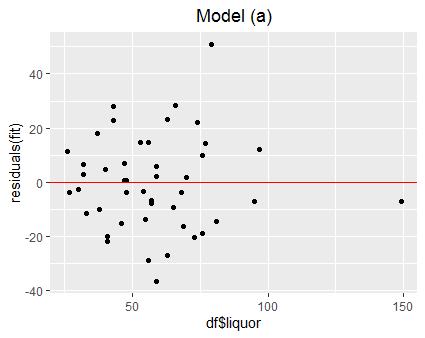
\includegraphics[width=\linewidth]{Q4_8_1.png}
  \end{subfigure}
  \begin{subfigure}[h]{0.4\linewidth}
    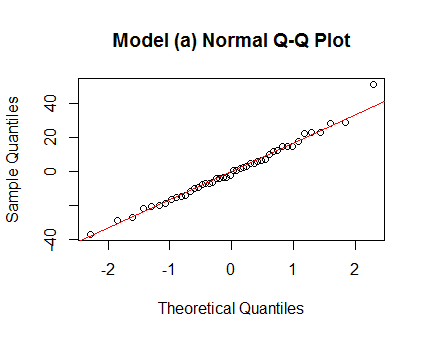
\includegraphics[width=\linewidth]{Q4_8_2.png}
  \end{subfigure}
\end{figure}

From the first plot, we can see there is no pattern of residuals. That is, residual is not a function of liquor consumption. From the second plot, we can see that the residuals belong to a normal distribution, since almost all points are on the line. Thus we think it is reasonable to assume that errors are $i.i.d.$ normal.

%4.9
\item
\verbatiminput{Q4_9_1.txt}
Therefore the exact 95\% CI  for $\beta$ is [0.486901, 0.9575696]. \par
\vspace{0.4cm}
If the error is not normal, the estimator is still asymptotically normally distributed. In point 5, we have already got that the standard error of $\beta$ is 0.1168. We also know that $z_{0.975}=1.96$ and $\hat{\beta}=0.7222$. Therefore the asymptotic 95\% CI is [0.7222-1.96*0.1168, 0.7222+1.96*0.1168]. That is, [0.493272, 0.951128].

When the errors are normal, the exact CI should be used. It is wider than the asymptotic CI, so it is a more conservative and safer way of inference. \par
The asymptotic CI also works when the errors are not normal and the sample size is very large. 


%4.10
\item
The confidence interval of bootstrapping method is [0.5511782, 0.9791503], which is very similar to the CIs obtained above. Generally speaking, the bootstrapped CI is not stable.
\begin{center}
  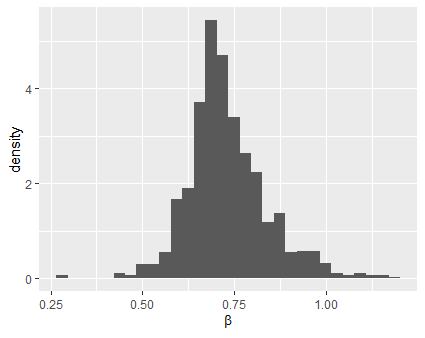
\includegraphics[width=0.7\linewidth]{Q4_10.png}
\end{center}

%4.11
\item
Part of the code and output is as follows. 
\verbatiminput{Q4_11.txt}

As we can see the $\hat{\rho}=0.6819694$. As for $\hat{\rho}_{(i)}-\hat{\rho}$, the minimum difference is around -0.066, and the maximum difference is around 0.021, so we do not think there are any observations that are particularly influential in the analysis. \par
FYI, the minimum difference is caused by $(y_{36},x_{36}) = (149, 122)$; the maximum difference is caused by $(y_{43},x_{43}) = (59,28)$

\end{enumerate}
\end{document}